\section{Investigation of Series and Parallel Connection}\label{sec:SimResults}

Modüler yapıya dair motivasyon (kısaca) %intro kısmında mevcut

\subsection{Series Connection}
The fundamental motivation behind series connection of inverter modules is the reduction of module DC bus voltage. It is persistently emphasized in \cite{Wang2013}, \cite{Zlwka} and \cite{Wang2015b} that the application of interleaving in series connection reduces the size of DC bus capacitors. However, it is not entirely true. The DC bus voltage ripple of each module along with total DC bus are shown in Fig. \ref{fig:series_volt_ripple}. It has been shown that interleaving only reduces the ripple on total DC bus ripple which has no positive effect on the system since the module voltages always has the ripple. Moreover, the capacitor ripple currents are not affected by interleaving since it is simply impossible to have a different current when modules are connected in series. For this very reason, the connection inductances between modules have no direct effect.

%% module dc bus voltages + dc bus/2 with interleaving (zoomed-faz kayması görünmeli)

\begin{figure}[tb]
\minipage{0.49\textwidth}
  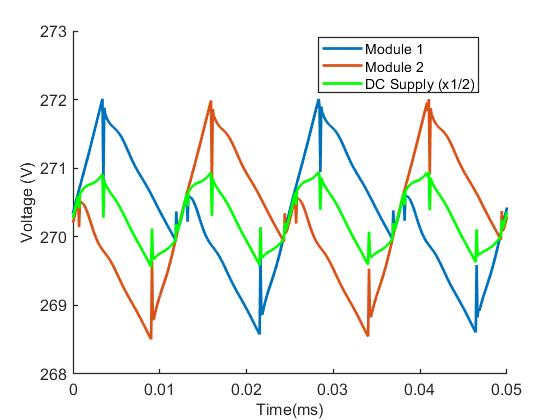
\includegraphics[width=\linewidth]{figures/series_volt_ripple.jpg}
  \caption{DC bus voltage ripple in series connected modules}\label{fig:series_volt_ripple}
\endminipage\hfill
\minipage{0.49\textwidth}
  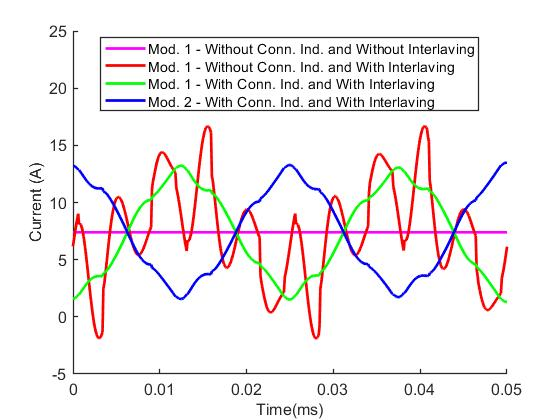
\includegraphics[width=\linewidth]{figures/parallel_current_trans.jpg}
  \caption{Current transition occuring due to interleaving in parallel connected modules}\label{fig:parallel_current_trans}
\endminipage
\end{figure}
% Fig.7 Caption REVIEW

\subsection{Parallel Connection}

The parallel connection is usually favored to reduce the size of DC bus capacitors with interleaving. However, when gate signals of two modules are phase shifted with proper angle, transition (circulating) currents between modules emerge, as shown in Fig. \ref{fig:parallel_current_trans}.

%% Zoomed olarak aşağıdaki üç akım gösterilecek:
%% Module-1 input akımı (DC bu) - no int - no ind
%% Module-1 input akımı (fsw etrafınmda osilasyon) - yes int - no ind
%% Module-2 input akımı (fsw etrafınmda osilasyon) - yes int - no ind
%% Module-1 input akımı (high freq ekleniyor) - yes int - yes ind
%% bu fig 6in yanına alınacak
%% vurguları gözden geçirelim !!!


The reduction on the capacitor current stress on the DC link capacitor currents when interleaving is applied in parallel connected modules has been shown for different number of modules and phase shift angles \cite{Ugur2017}. However, this analysis is only valid in ideal case where commutation and connection inductances are ignored. the voltage ripple is also expected to reduce in accordance. However, the results of the model which takes those parasitics into account suggest otherwise such that the application of interleaving may even worsen the situation. The voltage ripple and the current ripple of Dc bus capacitors with interleaving are shown in Fig. \ref{fig:parallel_volt_ripple} and Fig. \ref{fig:parallel_curr_ripple}, respectively. To better visualise the severity of the situation, the RMS of DC bus currents with and without interleaving are obtained for a full cycle of 3-phase currents and shown in Fig. \ref{parallel_curr_rms} for different phases.

Burada RMS akımları yorumlanacak (peak nerede oluyor vs.)

Akım geçişlerinin potansiyel problemleri ???

\begin{figure}[tb]
\minipage{0.49\textwidth}
  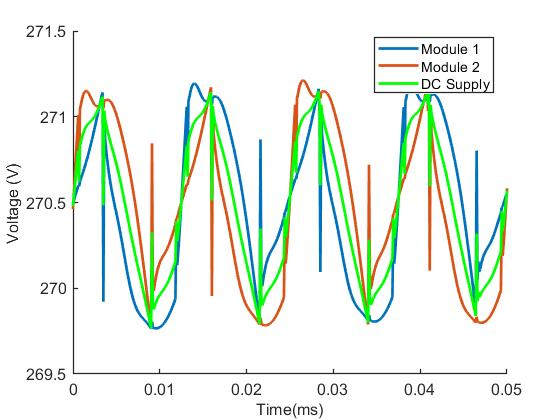
\includegraphics[width=\linewidth]{figures/parallel_volt_ripple.jpg}
  \caption{DC bus voltage ripple in parallel connected modules }\label{fig:parallel_volt_ripple}
\endminipage\hfill
\minipage{0.49\textwidth}
  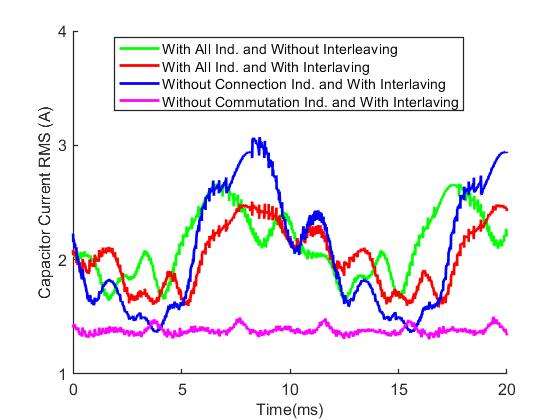
\includegraphics[width=\linewidth]{figures/parallel_curr_rms.jpg}
  \caption{Variation of DC bus capacitor current RMS in parallel connected modules}\label{fig:parallel_curr_rms}
\endminipage
\end{figure}


%% 4 akım rms variation:
%% No int yes ind (both) module 1 phase a cap
%% Yes int yes ind (both) module 1 phase a cap
%% Yes int yes ind (comm) module 1 phase a cap
%% Yes int yes ind (conn) module 1 phase a cap


\subsection{Discussions}

Serinin potansiyel sıkıntıları

Serinin avantajları ve dezavantajları

Seride interleaving aslında efektif olarak etken değil

Paralelde ideal durumdakinin daha bile kötüsüne gidebilir

Paralelin avantajları

Çok sayıda modül olsa ne olurdu (seri)

Çok sayıda modül olsa ne olurdu (paralel) - interleavin daha bile kötüleştirebilir- modüllerin nasıl bağlandığına bağlı
